%-----------------------------------------------------------------
%	BASIC DOCUMENT LAYOUT
%-----------------------------------------------------------------
\documentclass{beamer}

% \usepackage[scaled]{helvet}
% \renewcommand\familydefault{\sfdefault}
\usefonttheme[onlymath]{serif}

\usepackage[T1]{fontenc}
\usepackage[utf8]{inputenc}
\usepackage{microtype}
\usepackage[british]{babel}
\usepackage{url}
\usepackage{ru-theme}

\usepackage[backend=bibtex, style=trad-abbrv, sorting=none, maxbibnames=3, maxcitenames=2]{biblatex}
\addbibresource{bibliography.bib}
\makeatletter
	\def\blx@maxline{77}
\makeatother

\usepackage{array}
\usepackage{multirow}

\usepackage{multimedia}

%-----------------------------------------------------------------
%	MISC STUFF
%-----------------------------------------------------------------
\definecolor{mygreen}{RGB}{46,139,87}
\definecolor{mybrown}{RGB}{136,58,19}
\definecolor{myorange}{RGB}{241,122,60}

\newcommand{\Plus}{\mathord{\begin{tikzpicture}[baseline=0ex, line width=1, scale=0.13]
\draw (1,0) -- (1,2);
\draw (0,1) -- (2,1);
\end{tikzpicture}}}

\setbeamercovered{transparent}
\usepackage{tabularx}
\usepackage{float}
\usepackage{booktabs}
\usepackage{subfig}
% \usepackage{subcaption}

\usepackage{tikz}
\usetikzlibrary{shapes,arrows}
% Theorem environment	
\usepackage{amsthm}
\newtheorem{mydef}{Definition}
\newtheorem{myprop}{Proposition}
\newtheorem{mythm}{Theorem}
\newtheorem{mylem}{Lemma}
\newtheorem{mycor}{Corollary}
\newtheorem{myrem}{Remark}
\DeclareMathOperator{\Det}{det}
\DeclareMathOperator{\im}{im}
\DeclareMathOperator{\Rank}{rank}
\DeclareMathOperator{\Deg}{deg}

\AtBeginBibliography{\footnotesize}

%-----------------------------------------------------------------
%	LISTINGS
%-----------------------------------------------------------------
% \makeatletter

% \newcount\bt@rangea
% \newcount\bt@rangeb

% \newcommand\btIfInRange[2]{%
%     \global\let\bt@inrange\@secondoftwo%
%     \edef\bt@rangelist{#2}%
%     \foreach \range in \bt@rangelist {%
%         \afterassignment\bt@getrangeb%
%         \bt@rangea=0\range\relax%
%         \pgfmathtruncatemacro\result{ ( #1 >= \bt@rangea) && (#1 <= \bt@rangeb) }%
%         \ifnum\result=1\relax%
%             \breakforeach%
%             \global\let\bt@inrange\@firstoftwo%
%         \fi%
%     }%
%     \bt@inrange%
% }
% \newcommand\bt@getrangeb{%
%     \@ifnextchar\relax%
%         {\bt@rangeb=\bt@rangea}%
%         {\@getrangeb}%
% }
% \def\@getrangeb-#1\relax{%
%     \ifx\relax#1\relax%
%         \bt@rangeb=100000%   \maxdimen is too large for pgfmath
%     \else%
%         \bt@rangeb=#1\relax%
%     \fi%
% }

% \newcommand<>{\btLstHL}[1]{%
%   \only#2{\btIfInRange{\value{lstnumber}}{#1}{\color{orange!30}\def\lst@linebgrdcmd{\color@block}}{\def\lst@linebgrdcmd####1####2####3{}}}%
% }%
% \makeatother

% \makeatletter
% \newenvironment{btHighlight}[1][]
% {\begingroup\tikzset{bt@Highlight@par/.style={#1}}\begin{lrbox}{\@tempboxa}}
% {\end{lrbox}\bt@HL@box[bt@Highlight@par]{\@tempboxa}\endgroup}

% \newcommand\btHL[1][]{%
%   \begin{btHighlight}[#1]\bgroup\aftergroup\bt@HL@endenv%
% }
% \def\bt@HL@endenv{%
%   \end{btHighlight}%
%   \egroup
% }
% \newcommand{\bt@HL@box}[2][]{%
%   \tikz[#1]{%
%     \pgfpathrectangle{\pgfpoint{1pt}{0pt}}{\pgfpoint{\wd #2}{\ht #2}}%
%     \pgfusepath{use as bounding box}%
%     \node[anchor=base west, fill=orange!30,outer sep=0pt,inner xsep=1pt, inner ysep=0pt, rounded corners=3pt, minimum height=\ht\strutbox+1pt,#1]{\raisebox{1pt}{\strut}\strut\usebox{#2}};
%   }%
% }
% \makeatother

\usepackage[formats]{listings}
\usepackage{relsize}
\usepackage{chngcntr}
% \usepackage{lstlinebgrd}

\definecolor{keywords}{HTML}{268bd2}
\definecolor{background}{HTML}{eee8d5}
\definecolor{comments}{HTML}{586e75}

\lstdefinelanguage{mymatlab}[]{matlab}{%
	morekeywords={ss, lsim, place, rscale, curve1, curve2, curve3, curve4}
	}

\lstloadlanguages{matlab,python}
\lstset{language=matlab,
		basicstyle=\smaller\ttfamily,
		% keywordstyle=\bfseries,
		% morecomment=[l][\color{magenta}]{\#},
		keywordstyle=\color{keywords},
		commentstyle=\color{comments}\itshape,
		% backgroundcolor=\color{background},
		frame=tb,
		tabsize=2,
		breaklines=true,
		breakatwhitespace=true,
		numbers=left,
		numberstyle=\tiny,
		numbersep=7.5pt,
		xleftmargin=3ex}
\lstset{escapeinside={(*}{*)}}

% \lstset{language=matlab,
% 		frame=tb,
% 		% captionpos=b,
% 		tabsize=2,
% 		% showtabs=true,
% 		breaklines=true,
% 		breakatwhitespace=true,
% 		basicstyle=\smaller\ttfamily,
% 		numbers=left,
% 		numberstyle=\tiny,
% 		numbersep=7.5pt,
% 		% commentstyle=\textsl,
% 		xleftmargin=3ex}
% \lstset{escapeinside={(*}{*)}}   % for (*\ref{ }*) inside lstlistings (Scode)

\expandafter\patchcmd\csname \string\lstinline\endcsname{%
	\leavevmode
	\bgroup
}{%
	\leavevmode
	\ifmmode\hbox\fi
	\bgroup
}{}{%
	\typeout{Patching of \string\lstinline\space failed!}%
}
%% end of patch

\newcommand*{\inline}{\lstinline[basicstyle=\normalsize\ttfamily]}

%-----------------------------------------------------------------
%	MATHS AND SCIENCE
%-----------------------------------------------------------------
\usepackage{amsmath,amsfonts,amsthm,amssymb}
\usepackage{xfrac}
\usepackage[a]{esvect}
\usepackage{chemformula}
\usepackage{graphicx}

\usepackage[arrowdel]{physics}
	\renewcommand{\vnabla}{\vec{\nabla}}
	\renewcommand{\vectorarrow}[1]{\vec{#1}}
	\renewcommand{\vectorunit}[1]{\hat{#1}}
	\renewcommand*{\grad}[1]{\vnabla #1}
	\renewcommand*{\div}[1]{\vnabla \vdot \va{#1}}
	\renewcommand*{\curl}[1]{\vnabla \cp \va{#1}}
	\let\rot\curl

% SI units
\usepackage[separate-uncertainty=true]{siunitx}
\sisetup{range-phrase = \text{--}, range-units = single}
\DeclareSIPrePower\quartic{4}

%-----------------------------------------------------------------
%	PDF INFO AND HYPERREF
%-----------------------------------------------------------------
\usepackage{hyperref}
% \hypersetup{colorlinks, citecolor=black, filecolor=black, linkcolor=black, urlcolor=black}
\usepackage{cleveref}
	\crefname{section}{\S}{\SS}
	\Crefname{section}{\S}{\SS}
	\crefname{listing}{snippet}{}

\newcommand*{\mytitle}{Control of a Trailer}
\newcommand*{\myshorttitle}{Control of a Trailer}
\newcommand*{\mysubtitle}{How to steer a car when parking}
\newcommand*{\myauthor}{Alfredo Hernández}
\newcommand*{\myauthora}{David Masip}
\newcommand*{\myauthorb}{Martí Municoy}
\newcommand*{\myauthorc}{Jan-Hendrik Niemann}
\newcommand*{\myuni}{Universitat Autònoma de Barcelona}
\newcommand*{\mydegree}{Modelling for Science and Engineering}
\newcommand*{\mydate}{2nd February 2018}

\pdfstringdefDisableCommands{\def\and{and }}

\usepackage{hyperxmp}
% \hypersetup{pdfauthor={\myauthor}, pdftitle={\mytitle: \mysubtitle}}
\hypersetup{pdfauthor={\myauthor}, pdftitle={\mytitle}}

%-----------------------------------------------------------------
%	TITLE SECTION AND DOCUMENT BEGINNING
%-----------------------------------------------------------------

\title[\mytitle]{\mytitle}

\subtitle{\mysubtitle}

\author[Team 7]{ \myauthor \and \myauthora \and \myauthorb \and \myauthorc }% \and \myauthora \and \myauthorb \and \myauthorc}

% \institute[]{\myuni { --} \mydegree}
\institute[]{\mydegree}

\date[\mydate]{\mydate}

\hypersetup{pdfauthor={\myauthor}, pdftitle={\mytitle: \mysubtitle}}

\begin{document}

\begin{frame}
	\titlepage
\end{frame}

%-----------------------------------------------------------------
%	DOCUMENT BODY
%-----------------------------------------------------------------
% \begin{frame}
% 	\frametitle{Outline}
% 	\tableofcontents
% \end{frame}

%-----------------------------------------------------------------
%	INTRODUCTION
%	!TEX root = ./main.tex
%-----------------------------------------------------------------
\section{Introduction}

%-------------------------------
\subsection{The Problem}
\begin{frame}{Modelling the Kinematics I}
\begin{minipage}{.4\textwidth}
    \begin{figure}[H]
        \centering
        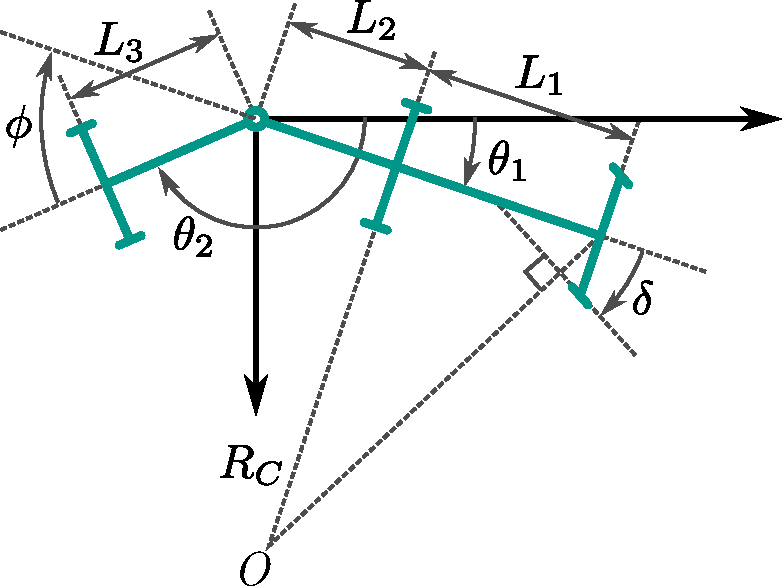
\includegraphics[width=\textwidth]{images/trailer-diagram}
        \caption{Geometric model of the car-trailer system}
        \label{fig:geom-model}
    \end{figure}
\end{minipage}%
\begin{minipage}{0.6\textwidth}
    \begin{table}[H]
        \tiny
        \centering
        \begin{tabularx}{0.95\textwidth}{c X}
            \toprule
            \toprule
            Parameters & Description \\
            \midrule
            $\theta_{1}$  & Angle of the car. \\
            $\theta_{2}$  & Angle of the trailer. \\
            $\phi$        & Angle between car and trailer. \\
            $\delta$      & Steering angle. \\
            $V$           & Speed of the car. \\
            $V_{trailer}$ & Speed of the trailer. \\
            $R_{C}$       & Distance from the centre of rotation $O$ to rear axle of the car. \\
            $L_{1}$       & Wheelbase of the car. \\
            $L_{2}$       & Overhang from the rear axle of the car to the hitch point. \\ 
            $L_{3}$       & Distance from the trailer axle to the hitch. \\ 
            \bottomrule
        \end{tabularx}
        \caption{Physical parameters of the system described by our model}
        \label{tab:parameters}
    \end{table}
\end{minipage}
\end{frame}

\begin{frame}{Modelling the Kinematics II}
\begin{minipage}{.4\textwidth}
    \begin{figure}[H]
        \centering
        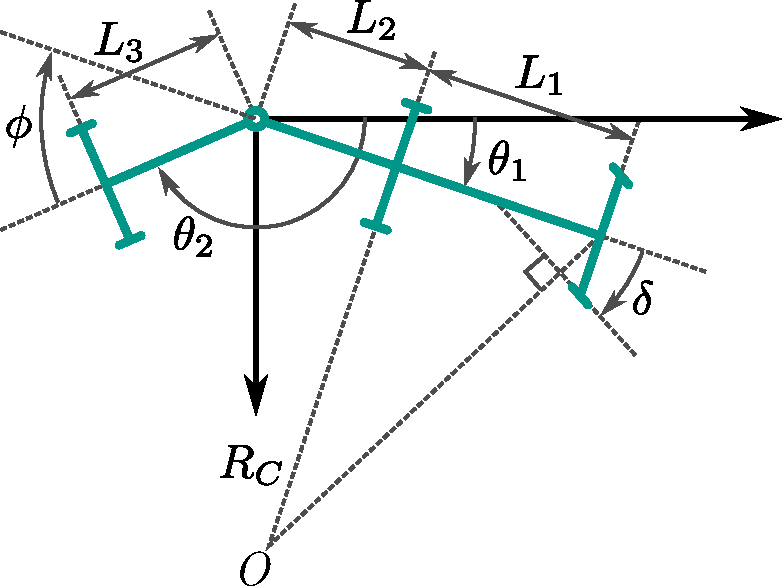
\includegraphics[width=\textwidth]{images/trailer-diagram}
        \caption{Geometric model of the car-trailer system}
        \label{fig:geom-model}
    \end{figure}
\end{minipage}%
\begin{minipage}{0.55\textwidth}
    \footnotesize
    \begin{onlyenv}<1->
    \begin{align*}
        \phi = \pi - (\theta_{2} - \theta_{1}) \qc
        \dot{\phi} = -\dot{\theta}_{2} + \dot{\theta}_{1} 
    \end{align*}
    \end{onlyenv}
    \begin{onlyenv}<+>
    \begin{align*}
        \dot{\theta}_{1} = -\frac{V}{R_{C}} \qc 
        R_C = \frac{\tan \delta}{L_1}
    \end{align*}
    \end{onlyenv}
    \begin{onlyenv}<+->
    \begin{align*}
        \dot{\theta}_{1} = -\frac{V}{L_{1}} \tan \delta 
    \end{align*}
    \end{onlyenv}
    % \begin{onlyenv}<4>
    % \begin{align*}
    %     V_{trailer} = -L_{2} \dot{\theta}_{1} \sin \phi + V \cos \phi
    % \end{align*}
    % \end{onlyenv}
    \begin{onlyenv}<+->
    \begin{align*}
        \dot{\theta}_{2} =  \frac{L_{2} \dot{\theta}_{1} \cos \phi + V \sin \phi }{L_{3}}
    \end{align*}
    \end{onlyenv}
\end{minipage}
\begin{onlyenv}<+->
\begin{align}\label{eq:dotphi-final}
    \dot{\phi} = - \frac{V}{L_{3}} \sin \phi - \frac{V}{L_{1}} \tan \delta \qty( 1 + \frac{L_{2}}{L_{3}} \cos \phi )
\end{align}
\end{onlyenv}
    
\end{frame}

%-------------------------------
\subsection{Approach}
\begin{frame}{Approaches to Solving the Problem}
\begin{itemize}
    \item Controller using pole placement
    \item Optimisation-based control
    \item Steering-based control
\end{itemize}

\end{frame}
%-----------------------------------------------------------------
%	CONTROL THEORY
%	!TEX root = ./main.tex
%-----------------------------------------------------------------
\section{Introduction to Control Theory}

%-----------------------------------------------------------------
\subsection{Control Theory}
\begin{frame}

\begin{onlyenv}<1>
\only{\frametitle{What is Control Theory?}}<1>
	\tikzstyle{block} = [draw, fill=white, rectangle,minimum height=3em, minimum width=6em]
	\tikzstyle{sum} = [draw, fill=white, circle, node distance=1cm]
	\tikzstyle{input} = [coordinate]
	\tikzstyle{output} = [coordinate]
	\tikzstyle{pinstyle} = [pin edge={to-,thin,black}]	
	\begin{figure}[h]
		\centering
		\begin{tikzpicture}[auto, node distance=4cm,>=latex']
		\node [input, name=input] {};
		\node [block, right of=input,node distance=4cm] (system) {Dynamical System};
		\draw [->] (input) -- node[name=u] {$u$} (system);
		\node [output, right of=system] (output) {};
		\draw [->] (system) -- node [name=y] {$y$}(output);
		\end{tikzpicture}
		\caption{Block diagram of a dynamical system}
		\label{fig:blockdiagram_dyn_sys}
	\end{figure}
	\begin{itemize}
		\item Input $u(t)$ which represents controls, noises and disturbances
		\item Output $y(t)$ representing the measurements
		\item Assumption: approximation by \begin{align}\label{eq:dynsys}
		\begin{split}
		\dot{x}(t) &= f(t, x(t), u(t))\\
		\dot{y}(t) &= h(x(t), u(t))
		\end{split}
		\end{align}
	\end{itemize}
\end{onlyenv}
% \end{frame}

% \begin{frame}{What is Control Theory?}
\begin{onlyenv}<2>
\only{\frametitle{What is Control Theory?}}<2>
\begin{itemize}
	\item Consider system (\ref{eq:dynsys}) is a \emph{linear time-invariant control system} of the form
	\begin{align}\label{eq:LTI}
	\begin{aligned}
		\dot{x}(t) &= Ax(t) + Bu(t)\\
		\dot{y}(t) &= Cx(t) + Du(t)
	\end{aligned}
	\end{align}
	\item \emph{System matrix} $A$, \emph{input matrix} $B$, \emph{output matrix} $C$ and \emph{feed-through matrix} $D$
	\item When a nonlinear system is given (3) is obtained by linearisation at points $(x^*,u^*)$ such that $f(x^*,u^*) = 0$
\end{itemize}
\end{onlyenv}

\end{frame}

%-----------------------------------------------------------------
\subsection{Controllability}

\begin{frame}

\begin{onlyenv}<1>
% \begin{frame}
\only{\frametitle{What is Controllability?}}<1>
	Simply said, a system is said to be controllable if it is possible to find a control input that takes the system from any initial state to any final state in any given time interval.
% \end{frame}
\end{onlyenv}

\begin{onlyenv}<2>
% \begin{frame}
\only{\frametitle{Controllability: Definition - Reachable \& Controllable}}<2>
	\begin{mydef}
		A system $(A,B)$ is called
		\begin{itemize}
			\item \emph{reachable} at time $T > 0$ if for all $x^1 \in \mathbb{R}^n$ there exists $(x,u)\in\mathcal{B}_{(A,B)}$ such that $x(0) = 0$ and $x(T) = x^1$
			\item \emph{controllable} at time T if for all $x^0,x^1 \in \mathbb{R}^n$ there exists $(x,u)\in\mathcal{B}_{(A,B)}$ such that $x(0) = x^0$ and $x(T) = x^1$
			\item \emph{null-controllable} at time T if for all $x^0 \in \mathbb{R}^n$ there exists $(x,u)\in\mathcal{B}_{(A,B)}$ such that $x(0) = x^0$ and $x(T) = 0$.
		\end{itemize}
	\end{mydef}
% \end{frame}
\end{onlyenv}

\begin{onlyenv}<3>
\only{\frametitle{Controllability: Definition - Simply said}}<3>
	\emph{Reachable} means that we can steer the system from 0 to any final state in any time $Z$. \emph{Controllable} mean that it is possible to steer the system from any initial state to any final state in any given time $T$ and hence \emph{null-controllable} means that the final state is 0.
% \end{frame}
\end{onlyenv}

%\begin{frame}{Controllability: Definition - Reachable \& Controllable Set}
%\begin{mydef}
%	The \emph{reachable set} from $x^0 \in \mathbb{R}^n$ at time $T>0$ is defined as
%	\begin{align*}
%	\mathcal{R}_{x^0}(T) := \{x^1 \in \mathbb{R}^n \mid \exists (x,u) \in \mathcal{B}_{(A,B)}: x(0) = x^0, x(T) = x^1   \}.
%	\end{align*}\\The \emph{controllable set} to $x^1\in\mathbb{R}^n$ at time $T$ is defined as
%	\begin{align*}
%	\mathcal{C}_{x^1}(T) := \{x^0 \in \mathbb{R}^n \mid \exists (x,u) \in \mathcal{B}_{(A,B)}: x(0) = x^0, x(T) = x^1   \}.
%	\end{align*}
%\end{mydef}
%\end{frame}

\begin{onlyenv}<4>
\only{\frametitle{Controllable: Yes or No?}}<4>
	\begin{mythm}
		For all $T>0$ it holds
		\begin{align*}
		\mathcal{R}_0(T) = \im[B,AB,...,A^{n-1}B]   =: K(A,B) \in \mathbb{R}^{n \times nm}.
		\end{align*}
	\end{mythm}
	\begin{mycor}\label{cor:ctrb}
		For a system $(A,B)$ the following statements are equivalent:
		\begin{enumerate}
			\item There exists $T>0$ such that $(A,B)$ is controllable at time $T$.
			\item $\im(K(A,B)) = \mathbb{R}^n$
			\item $\Rank(K(A,B)) = n$
			\item For all $T>0$ the system $(A,B)$ is controllable at time $T$. We say that $(A,B)$ is controllable.
		\end{enumerate}
	\end{mycor}
\end{onlyenv}

\end{frame}

%-------------------------------
\subsection{Pole Placement Theorem}

\begin{frame}
\begin{onlyenv}<1>
\only{\frametitle{Stability}}<1>
	\begin{itemize}
		\item From theory of differential equations stability of a system can be analysed by considering the eigenvalues of the matrix $A$
		\item One aim of control theory is stabilisation
	\end{itemize}
	\begin{alertblock}{Questions}
		What have eigenvalues and controllability in common?\\
		How can we stabilise a given system if possible?
	\end{alertblock}
% \end{frame}
\end{onlyenv}

\begin{onlyenv}<2>
\only{\frametitle{Stabilisation}}<2>

\tikzstyle{block} = [draw, fill=white, rectangle,minimum height=2em, minimum width=7em]
\tikzstyle{sum} = [draw, white, circle]
\tikzstyle{pinstyle} = [pin edge={to-,thin,black}]
\tikzstyle{input} = [coordinate]
\tikzstyle{output} = [coordinate]
	\begin{figure}
		\centering
		\begin{tikzpicture}[auto,node distance=2cm,>=latex']
		% We start by placing the blocks
		\node [input, name=input] {};
		\node [sum, right of=input] (sum) {};
		\node [block, right of=sum,align=center] (B) {$\dot{x}(t) = Ax(t) + Bu(t)$\\$\dot{y}(t) = Cx(t) + Du(t)$};
		\node [block, below of=B, align=center]  (K) {$\dot{\omega}(t) = K\omega(t) + Ly(t)$\\$\dot{u}(t) = M\omega(t) + Ny(t)$};
		\node [sum, right of=B] (sum2) {};
		\node [output, right of=sum2] (output) {};
		
		\draw [->] (input) -- node[name=sum] {u} (B);
		\draw [->] (B) -- node[pos=0.7, name=y] {y} (output);
		\draw [->] (y) |- node {}(K);
		\draw [->] (K) -| node {}(sum);
		\end{tikzpicture}
		\caption{Block diagram of a feedback loop}
		\label{fig:blockdiagram_feedback_loop}
	\end{figure}
	Aim: determine a feedback controller such that
	\begin{align*}
	\begin{pmatrix}
	\dot{x}(t) \\
	\omega(t)
	\end{pmatrix} =
	\begin{pmatrix}
	A+BNC & BM \\
	LC & K
	\end{pmatrix}
	\begin{pmatrix}
	x(t) \\
	\omega(t)
	\end{pmatrix}
	\end{align*}
	is internally stable, i.e. all eigenvalues of A have negative real part.
% \end{frame}
\end{onlyenv}

\begin{onlyenv}<3>
\only{\frametitle{Pole Placement Theorem}}<3>
	\begin{mythm}\label{thm:PP}
		Let $(A,B)$ be a system as in (3). The the system is controllable if and only if for all monic, i.e. the leading coefficient is 1, polynomial $p(s) \in\mathbb{R}[s]$ with $\Deg(p(s)) = n$ there exists $F\in\mathbb{R}^{m\times n}$ such that $p(s) = \Det((A+BF)-sI)$.
	\end{mythm}
% \end{frame}
\end{onlyenv}

\begin{onlyenv}<4>
\only{\frametitle{Pole Placement Theorem - What does it say?}}<4>
	We see that if the system is controllable we can place the eigenvalues everywhere we like and therefore are able to stabilise our system.
\end{onlyenv}

\end{frame}

%-------------------------------
\subsection{Controller Design}

\begin{frame}

\begin{onlyenv}<1>
\only{\frametitle{Achieve Stability}}<1>
	\begin{itemize}
		\item Linearise the model about $\phi = 0$ and $\delta = 0$ using a Taylor series:
		\item We get
		\begin{align}\label{eq:controler-system}
		\Delta \dot{\phi} = \frac{V}{L_{3}} \Delta \phi - \frac{V}{L_{1}} \qty( 1 + \frac{L_{2}}{L_{3}} ) \Delta \delta 
		\end{align}
		with
		\begin{align*}
		\Delta \phi = \phi - \phi_{0} 
		\end{align*}
		\item $A=\frac{V}{L_3}$, $B = -\frac{V}{L_1}(1+\frac{L_2}{L_3})$, $x = \Delta\phi$ and $u=\Delta\delta$
		\item For $C$ we can choose 1 and therefore $y=x$ since $D=0$
	\end{itemize}
% \end{frame}
\end{onlyenv}

\begin{onlyenv}<2>
\only{\frametitle{Is it controllable?}}<2>
	\begin{itemize}
		\item Kalman-matrix is $K(A,B) = B$
		\item Since $B = -\frac{V}{L_1}(1+\frac{L_2}{L_3}) > 0$ is a positive scalar the Kalman-matrix has full rank and therefore the system is controllable
		\item We can use the pole placement theorem to stabilise the system
	\end{itemize}
% \end{frame}
\end{onlyenv}

\begin{onlyenv}<3>
\only{\frametitle{Full-State Feedback Controller}}<3>

\tikzstyle{block} = [draw, fill=white, rectangle, minimum height=3em, minimum width=3em]
\tikzstyle{sum} = [draw, fill=white, circle]
\tikzstyle{pinstyle} = [pin edge={to-,thin,black}]
\begin{figure}[h]
	\centering
	\resizebox{\textwidth}{!}{
	\begin{tikzpicture}[auto,node distance=1.5cm,>=latex']
	% We start by placing the blocks
	\node [input, name=input] {};
	\node [block,right of=input] (N) {$\bar{N}$};
	\node [sum, right of=N] (sum) {};
	\node [block, right of=sum] (B) {$B$};
	\node [sum, right of=B] (sum2) {};
	\node [block, right of=sum2] (integrator) {$\dfrac{1}{s}$};
	\node [block, right of=integrator, xshift=1cm] (C) {$C$};
	\node [block, below of=integrator] (A) {$A$};
	\node [block, below of=A] (K) {$K$};
	\node [output, right of=C] (output) {};
	
	\draw [->] (input) -- node {$r$} (N);
	\draw [->] (N) -- node[pos=0.7] {$+$} (sum);
	\draw [->] (sum) -- node {$u$} (B);
	\draw [->] (B) -- node[pos=0.7] {$+$} (sum2);
	\draw [->] (sum2) -- node {$\dot{x}$} (integrator);
	\draw [->] (integrator) -- node[name=x]  {$x$} (C);
	\draw [->] (C) -- node {$y$}(output);
	\draw [->] (A) -| node[pos=0.9] {$+$}(sum2);
	\draw [->] (x) |- node[pos=0.9] {}(A);
	\draw [->] (x) |- node[pos=0.9] {}(K);
	\draw [->] (K) -| node[pos=0.95] {$-$} (sum);
	\end{tikzpicture}}
	\caption{Block diagram of the state space model}
	\label{fig:gain-schedule}
\end{figure}
% \end{frame}
\end{onlyenv}

\begin{onlyenv}<4>
\only{\frametitle{Full-State Feedback Controller}}<4>
	For simplicity, let's assume the reference is zero, $r = 0$. The input is then
	\begin{align*}
	u = - K x
	\end{align*}
	The state-space equations for the closed-loop feedback system are, therefore,
	\begin{align}
	\begin{split}
	\dot{x} &= (A-BK) x\\
	y &= C x
	\end{split}\label{eq:systemX}
	\end{align}
% \end{frame}
\end{onlyenv}

%The stability and time-domain performance of the closed-loop feedback system are determined primarily by the location of the eigenvalues of the matrix ($A-BK$), which are equal to the closed-loop poles. Since the matrices $A$ and $BK$ are both $1\times 1$, there will be one pole for the system. By choosing an appropriate state-feedback gain matrix $K$, we can place these closed-loop poles anywhere we would like because the system is controllable. The pole placement theorem provides the theory that we can compute such a matrix $K$.

\begin{onlyenv}<5>
\only{\frametitle{Feedback matrix $K$}}<5>
	\begin{itemize}
		\item Stability and time-domain performance of the closed-loop feedback system are determined primarily by the location of the eigenvalues of the matrix ($A-BK$)
		\item We only have 1 eigenvale to place since our system is one dimensional
		\item[$\Rightarrow$] compute such a matrix $K$
	\end{itemize}
% \end{frame}
\end{onlyenv}

\begin{onlyenv}<6>
\only{\frametitle{Eliminate Steady State Error}}<6>
\begin{itemize}
	\item $\bar{N}$ is used to scale the reference input to make it equal to $K x$ in steady-state
	$\Rightarrow$ $K x$ will be equal to the desired output, i.e. that we do not get a non-zero steady state error
	\item $\bar{N}$ is computed in general as $\bar{N} = N_u + KN_x$ where $N_x = N(1:n)$ and $N_u = N(1+n)$ using MATLAB notation and
	\begin{align*}
	N = \begin{bmatrix}
	A & B \\ 
	C & D
	\end{bmatrix} ^{-1}
	\begin{bmatrix}
	0 \\ 
	1
	\end{bmatrix}
	\end{align*}
	where $[0,...,0,1]$ is a vector of size $n+1$, shortly represented as $[0,1]$, and $n$ the dimension of the system
\end{itemize}
\end{onlyenv}

\end{frame}
%-----------------------------------------------------------------
%	MODELS
%	!TEX root = ./main.tex
%-----------------------------------------------------------------
\section{Controller Implementation}

%-------------------------------
\subsection{Open-Loop Response}
\begin{frame}[fragile]{Open-Loop Response: Implementation}

\begin{lstlisting}[language=mymatlab]
% Time in seconds
t = 0:0.01:10;
% Input
u = zeros(size(t))*r;
% Create state space object
sys = ss(A,B,C,0);

% Calculate open-loop response
[y,t,x] = lsim(sys,u,t,phi_0);
\end{lstlisting}

\begin{itemize}
    \item \inline{ss()} defines the state space.
    \item \inline{lsim()} simulates the output time response $y(t)$ of dynamic system with input $u(t)$.
\end{itemize}
\end{frame}

\begin{frame}{Open-Loop Response: Simulation}
\begin{onlyenv}<1>
    \begin{figure}[H]
    	\centering
    	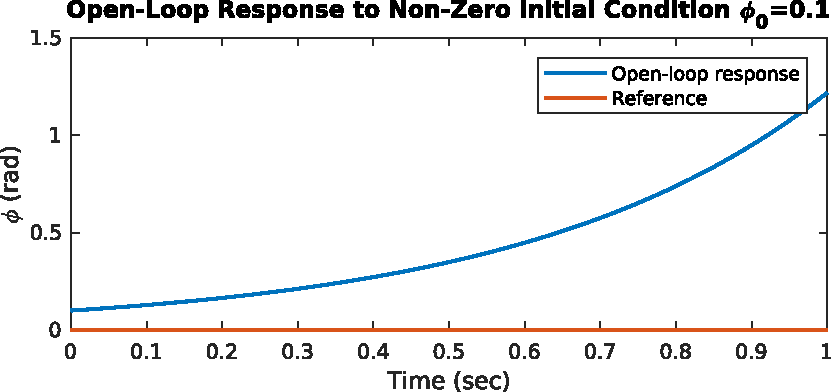
\includegraphics[width=0.7\textwidth]{images/curve-open-loop}
    	\caption{Open-Loop response to non-zero initial condition driving backwards with a trailer}
    	\label{fig:curve-open-loop}
    \end{figure}
\end{onlyenv}

\begin{onlyenv}<2>
    \begin{figure}[H]
    	\centering
    	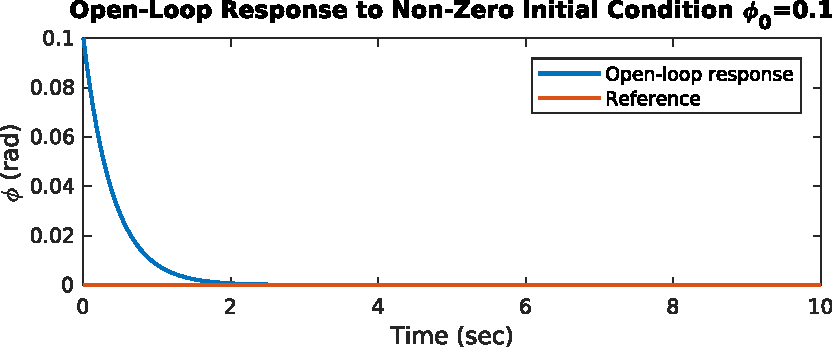
\includegraphics[width=0.73\textwidth]{images/stable-open-loop}
    	\caption{Open-Loop response to non-zero initial condition driving forwards with a trailer}
    	\label{fig:curve-open-loop-stable}
    \end{figure}
\end{onlyenv}
\end{frame}

%-------------------------------
\subsection{Closed-Loop Response}
\begin{frame}[fragile]{Closed-Loop Response: Implementation}

\begin{lstlisting}[language=mymatlab]
% Time in seconds
t = 0:0.01:60;
% Inputs
u = curve4(t, 0.4); % S shape
% Apply pole placement
K = place(A,B,-0.73);
% State space
sys_cl = ss(A-B*K,B,C,0);
% Calculate scaling factor
Nbar = rscale(sys,K);

% Calculate closed-loop response
[y_cl,t,x_cl] = lsim(sys_cl,Nbar*u,t,phi_0);
\end{lstlisting}

\begin{itemize}
    \item \inline{place()} finds the state-feedback gain $K$ and provides the desired closed-loop pole.
    \item \inline{rscale()} computes the desired scale factor $\bar{N}$.
\end{itemize}
\end{frame}

\begin{frame}{Closed-Loop Response: Simulation}
\begin{figure}[H]
	\centering
	\subfloat[Diagram of the curve]{%
		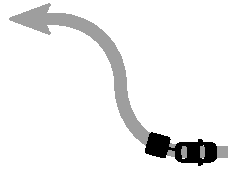
\includegraphics[height=0.15\textwidth]{images/curve4-diagram}%
		\label{fig:curve4a}%
		}%
	\hspace{0.5cm}%
	\subfloat[Closed-loop response of the controller]{%
		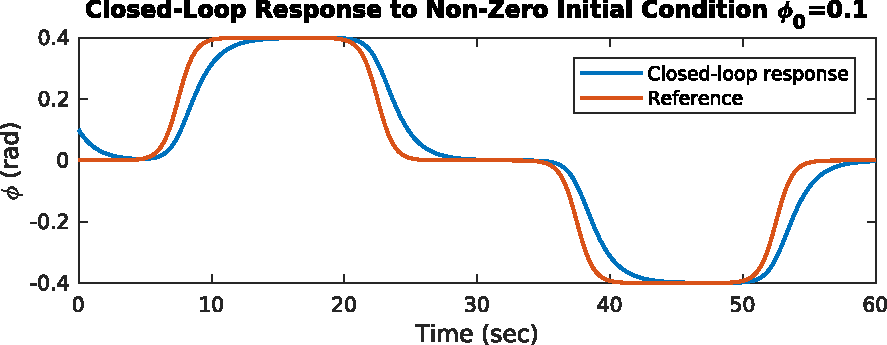
\includegraphics[height=0.28\textwidth]{images/control4-plot}%
		\label{fig:curve4b}%
		}%
	\caption{Diagram and control of the car-trailer system in a $S$-shaped curve}
\end{figure}

\footnotesize{Available at \url{https://github.com/aldomann/trailer-parking}}

\end{frame}

% \begin{frame}{Video test}
% 	\movie[width=10cm,height=6cm,poster]{Video}{videos/test.mp4}
% \end{frame}

%-----------------------------------------------------------------
%	STEERING CONTROL
%	!TEX root = ./main.tex
%-----------------------------------------------------------------
\section{Alternative Control Methods}

%-----------------------------------------------------------------
%	STEERING CONTROL
%	!TEX root = ./main.tex
%-----------------------------------------------------------------
\subsection{Optimisation-based}

\begin{frame}{Optimisation-based}

\begin{onlyenv}<1>
\begin{figure}[H]
    \centering
    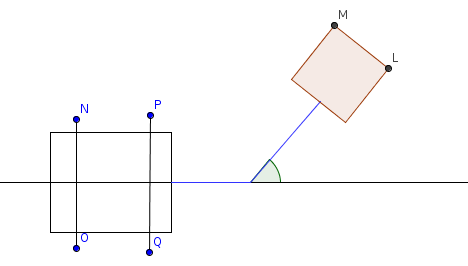
\includegraphics[width=0.55\textwidth]{images/pic_trailer.png}
    \caption{Geometric situation}
    \label{fig:trailer}
\end{figure}

\begin{figure}[H]
    \centering
    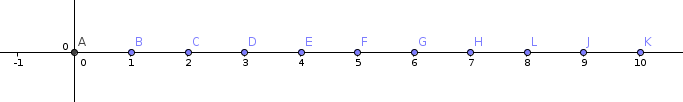
\includegraphics[width=0.55\textwidth]{images/divisions.png}
    \caption{Time divisions of the method}
    \label{fig:trailer2}
\end{figure}
% \end{frame}
\end{onlyenv}

% \begin{frame}{Frame Title}
\begin{onlyenv}<2>
We optimise, as a function of $\delta$:
\begin{align}
    \operatorname{cost}_{\alpha}(y, \phi) = y^2+\alpha \phi^2 
\end{align}

Solved using analytical expressions for the circular paths of the points in the car and using a Runge--Kutta--Fellberg 78 method to integrate the differential equation for $\phi$.
\end{onlyenv}

\begin{onlyenv}<3>
Issues with the method:
\begin{itemize}
    \item Greedy.
    \item Dependent on number of divisions and $\alpha$.
    \item One variable $\delta$ for two objectives ($y$, $\phi$).
\end{itemize}

\end{onlyenv}



\end{frame}



%-----------------------------------------------------------------
%	EXPERIENCE CONTROL
%	!TEX root = ./main.tex
%-----------------------------------------------------------------
%-----------------------------------------------------------------

\subsection{Steering-based Control}
\begin{frame}{The grounds of the approach}
\begin{minipage}{0.5\textwidth}
    \begin{figure}[H]
        \centering
        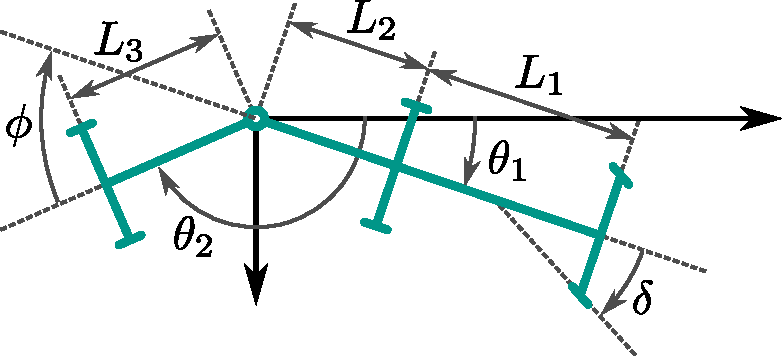
\includegraphics[width=\textwidth]{images/trailer-diagram-marti}
        % \caption{Geometric model of the car-trailer system}
        \label{fig:geom-model-marti}
    \end{figure}
\end{minipage}%
\hfill%
\begin{minipage}{0.5\textwidth}
\begin{itemize}
    \item Python 2.7 implementation
    \item Matplotlib
    \item NumPy
\end{itemize}
\end{minipage}

\begin{itemize}
    \item \footnotesize{$\dot{\phi} = \dfrac{V}{L_3} \cdot \sin{\phi} + \dfrac{V \cdot \tan{\delta}}{L_1} \cdot \left(1 + \dfrac{L_2 \cdot \cos{\phi}}{L_3}\right)$}
    \item \footnotesize{$\phi_i = \phi_{i-1} + \left( \dfrac{\sin{\phi_{i-1}}}{L_3} + \dfrac{\tan{\delta}}{L_1} \cdot \left( 1 + \dfrac{L_2 \cdot \cos{\phi_{i-1}}}{L_3}\right)\right) \cdot V \cdot \Delta t$}
\end{itemize}

2 main goals:
\begin{itemize}
    \item Visualise and check the behaviour of the model
    \item Create a steering-based controller
\end{itemize}
\end{frame}

\begin{frame}{First Tests of the Model}

\begin{onlyenv}<1>
\begin{minipage}{.5\textwidth}
    \begin{figure}[H]
        \centering
        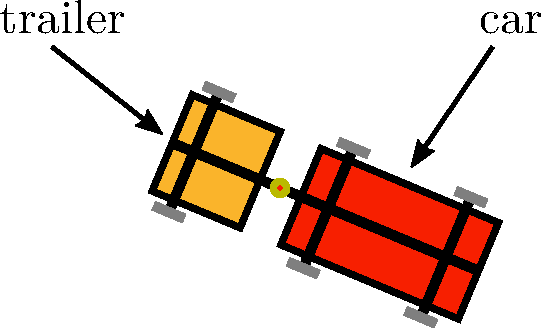
\includegraphics[width=0.6\textwidth]{images/car-trailer}
        \caption{Diagram of the system}
        \label{fig:car-trailer-diag}
    \end{figure}
    \begin{itemize}
        \item Go from $A$ to $B$ backwards.
    \end{itemize}
\end{minipage}%
\begin{minipage}{0.5\textwidth}
    \begin{figure}[H]
        \centering
        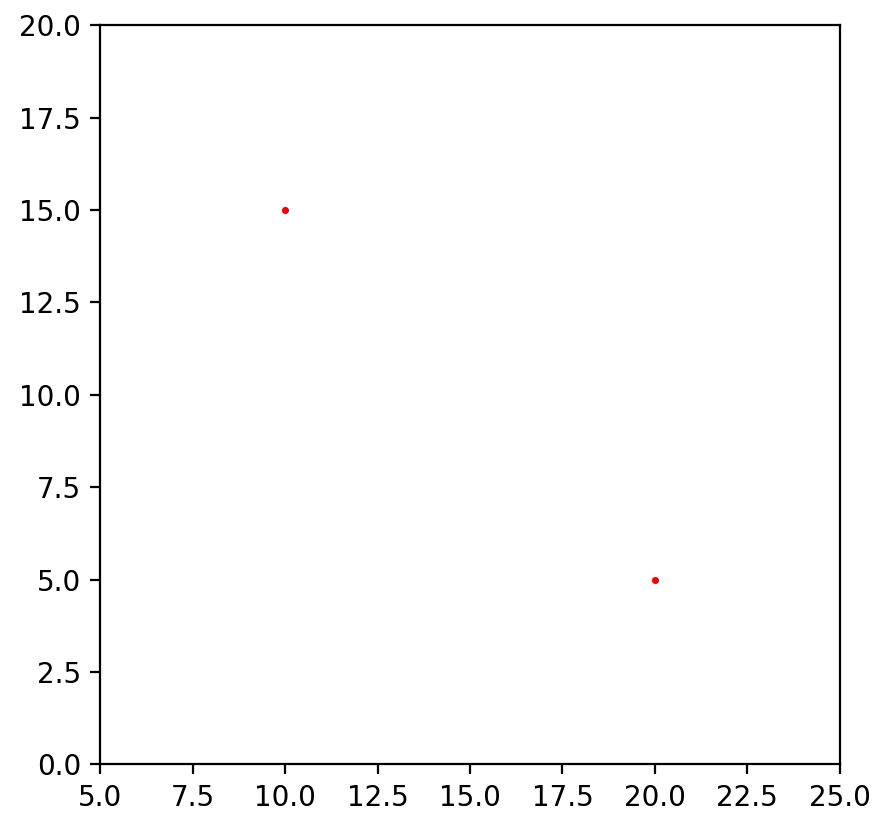
\includegraphics[width=\textwidth]{images/points}
        % \caption{Diagram of the system}
        \label{fig:points}
    \end{figure}
\end{minipage}
\end{onlyenv}

\begin{onlyenv}<2>
\begin{minipage}{.5\textwidth}
    \movie[width=6cm,height=4.5cm,poster]{%
        \hspace{0.8cm}%
        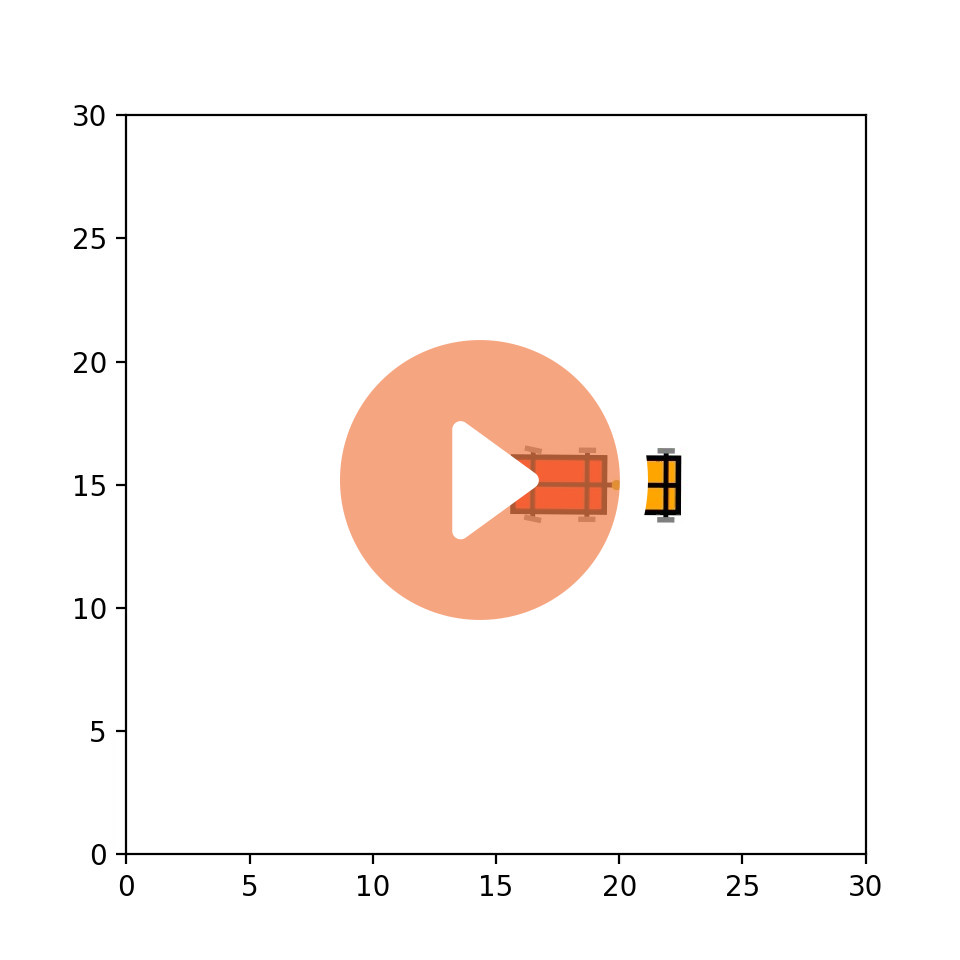
\includegraphics[width=0.8\textwidth]{images/thumbtest2}}%
        {videos/test2.mp4}
\end{minipage}%
\begin{minipage}{.5\textwidth}
    \movie[width=6cm,height=4.5cm,poster]{%
        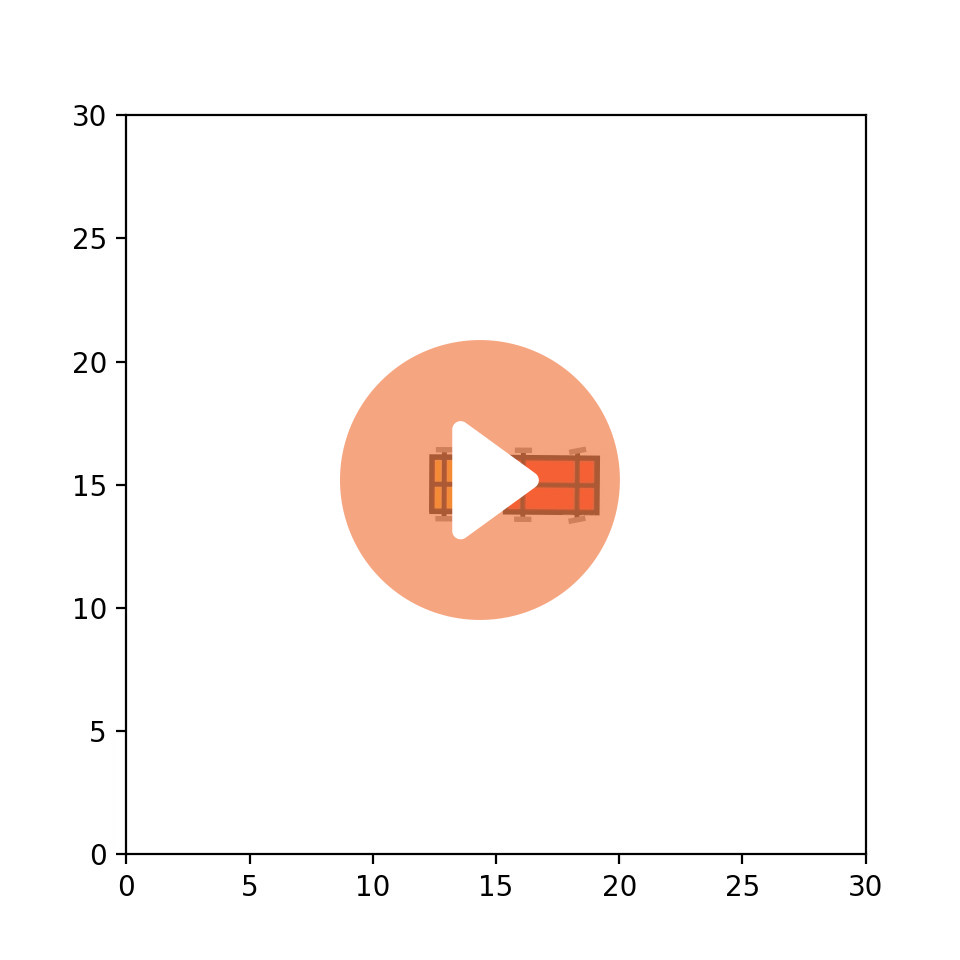
\includegraphics[width=0.8\textwidth]{images/thumbtest1}}%
        {videos/test.mp4}
\end{minipage}
\end{onlyenv}

\end{frame}

\begin{frame}{Steering-based Control}

\begin{onlyenv}<1-4>
\begin{minipage}{.45\textwidth}
    \begin{enumerate}[(i)]
        \footnotesize
        \item<2,4> Face trailer to a “non-annoying” direction.
        \item<3,4> Move the car to the goal point.
    \end{enumerate}
    \begin{itemize}
        \item<4> Keep repeating (i) until reaching point $B$.
    \end{itemize}
\end{minipage}%
\begin{minipage}{.55\textwidth}
    \begin{onlyenv}<1>
    \begin{figure}[H]
        \centering
        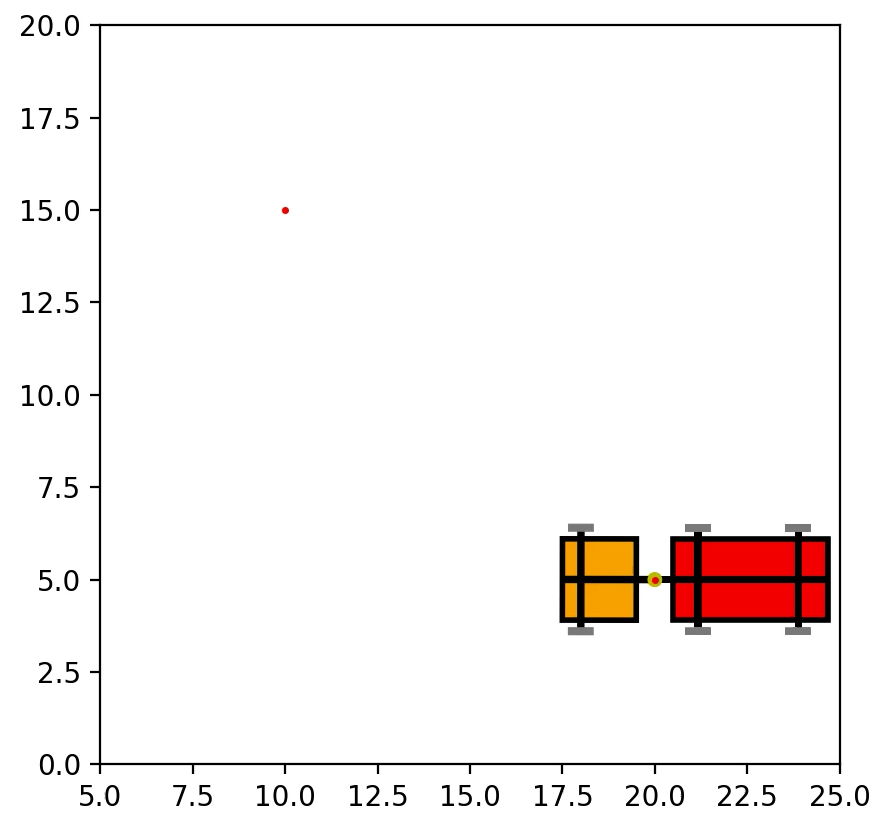
\includegraphics[width=\textwidth]{images/snapshot1}
        % \caption{Diagram of the system}
        \label{fig:points}
    \end{figure}
    \end{onlyenv}
    \begin{onlyenv}<2>
    \begin{figure}[H]
        \centering
        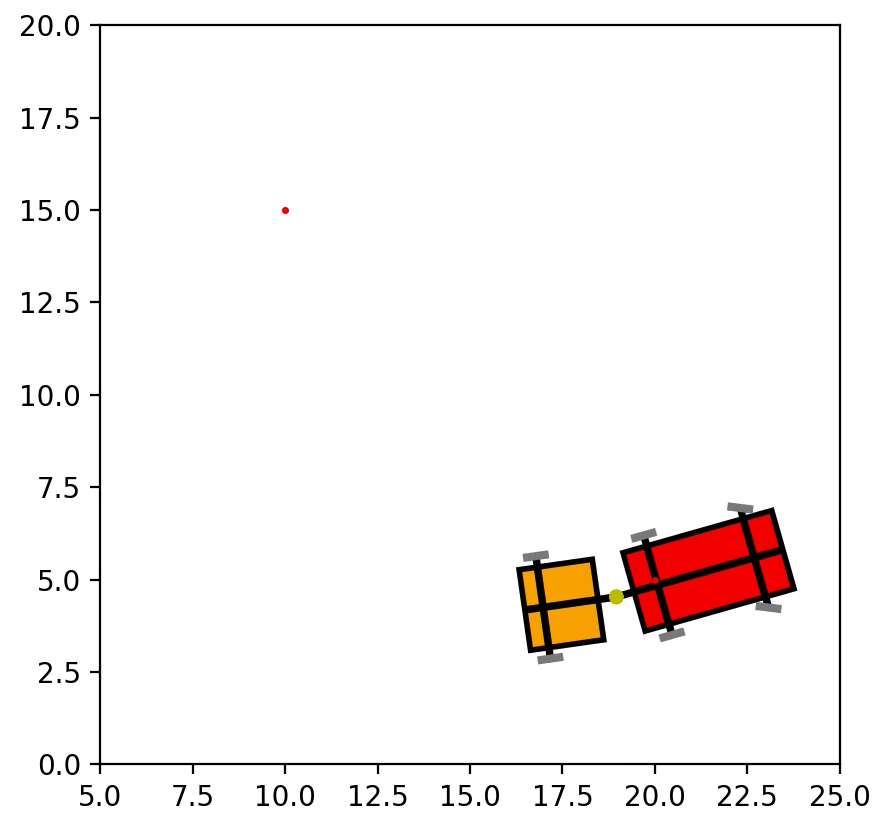
\includegraphics[width=\textwidth]{images/snapshot2}
        % \caption{Diagram of the system}
        \label{fig:points}
    \end{figure}
    \end{onlyenv}
    \begin{onlyenv}<3>
    \begin{figure}[H]
        \centering
        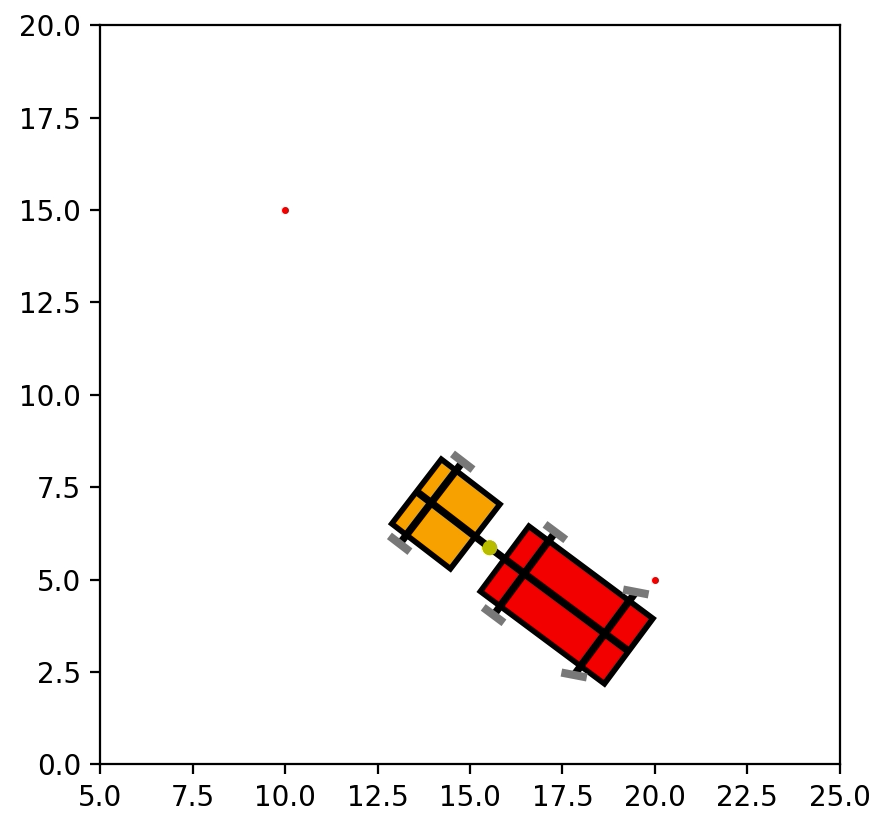
\includegraphics[width=\textwidth]{images/snapshot3}
        % \caption{Diagram of the system}
        \label{fig:points}
    \end{figure}
    \end{onlyenv}
    \begin{onlyenv}<4>
    \movie[width=7cm,height=5.25cm,poster]{%
        \hspace{0.8cm}%
        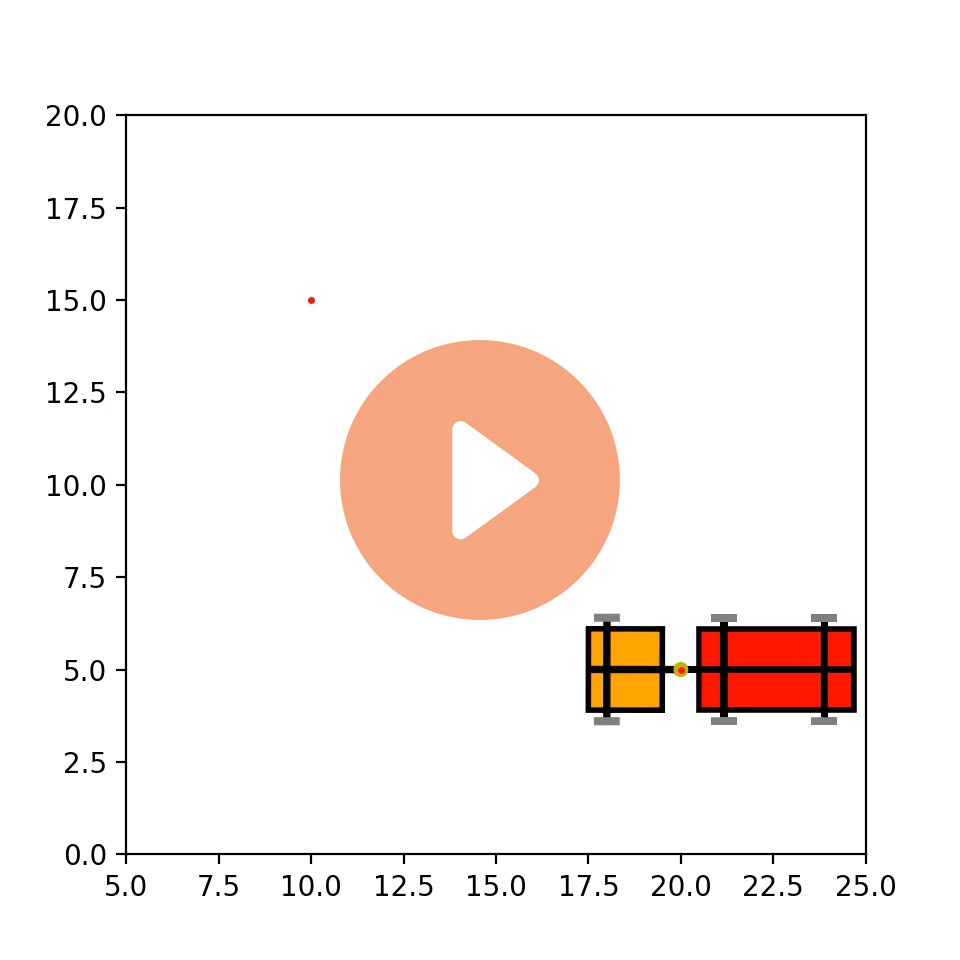
\includegraphics[width=0.8\textwidth]{images/thumb1}}%
        {videos/movie1.mp4}
    % \begin{figure}[H]
    %     \centering
    %     \movie[width=7cm,height=5.25cm,poster]{%
    %     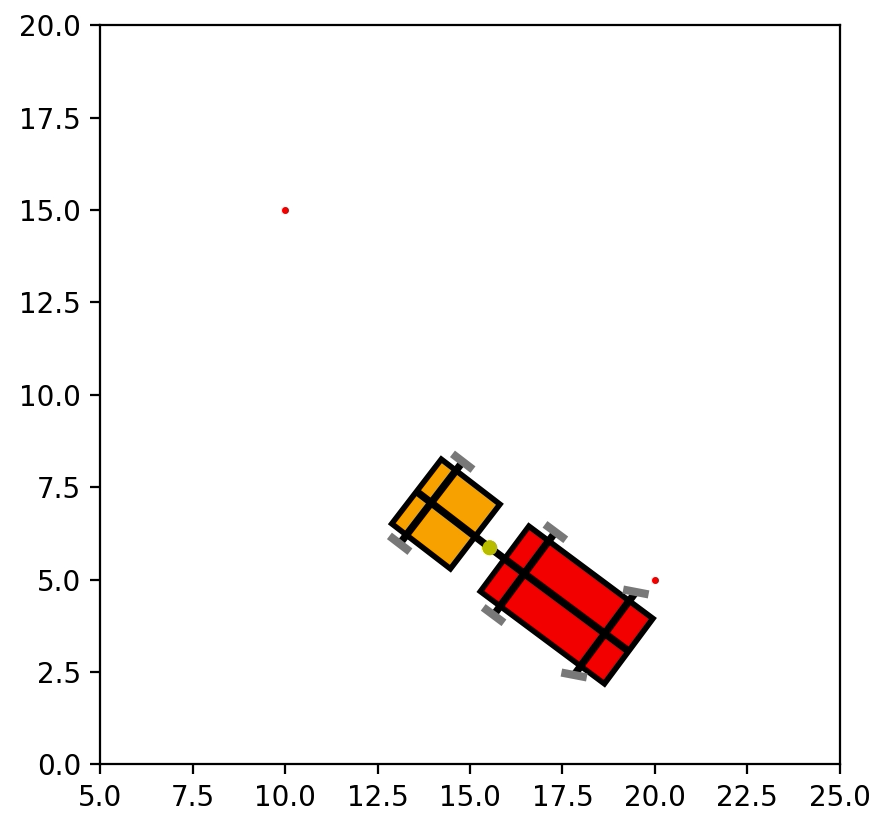
\includegraphics[width=\textwidth]{images/snapshot3}}%
    %     {videos/movie1.mp4}
    %     \label{fig:points}
    % \end{figure}
    \end{onlyenv}
\end{minipage}
\end{onlyenv}

\begin{onlyenv}<5>
\begin{minipage}{.5\textwidth}
    \movie[width=6cm,height=4.5cm,poster]{%
        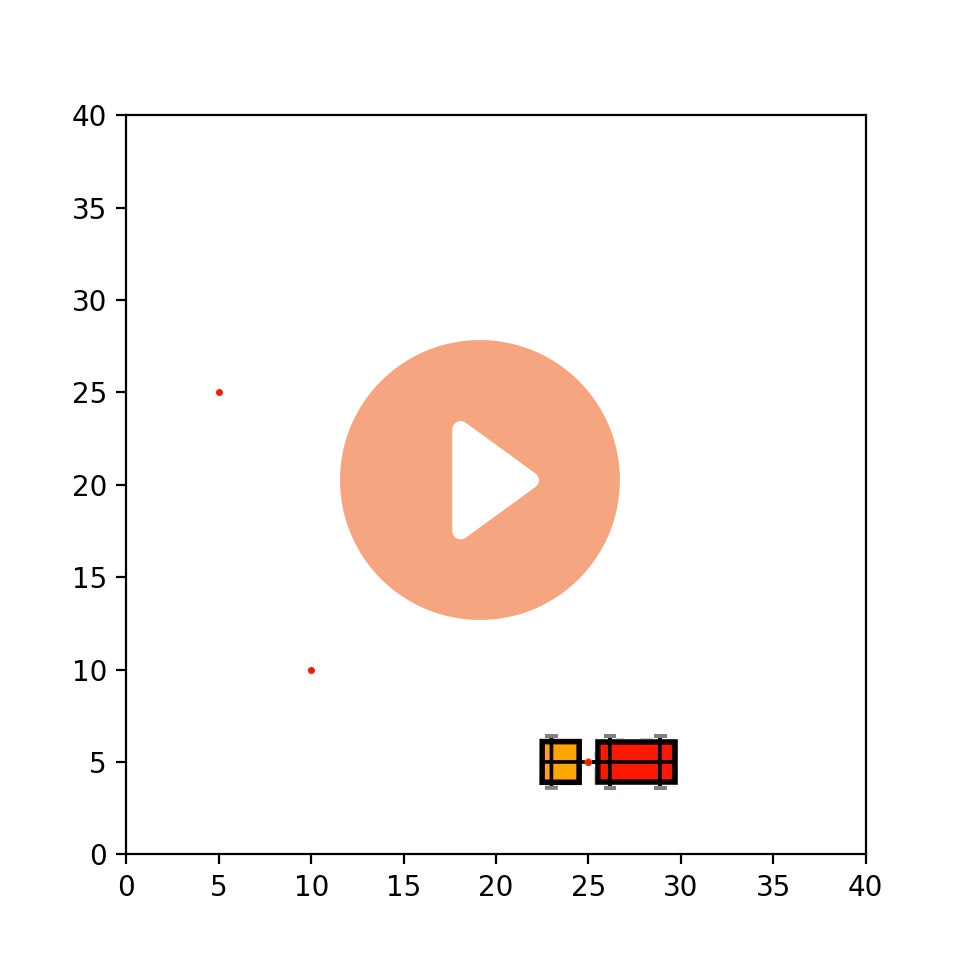
\includegraphics[width=0.8\textwidth]{images/thumb2}}%
        {videos/movie2.mp4}
\end{minipage}%
\begin{minipage}{.5\textwidth}
    \movie[width=6cm,height=4.5cm,poster]{%
        \hspace{0.8cm}%
        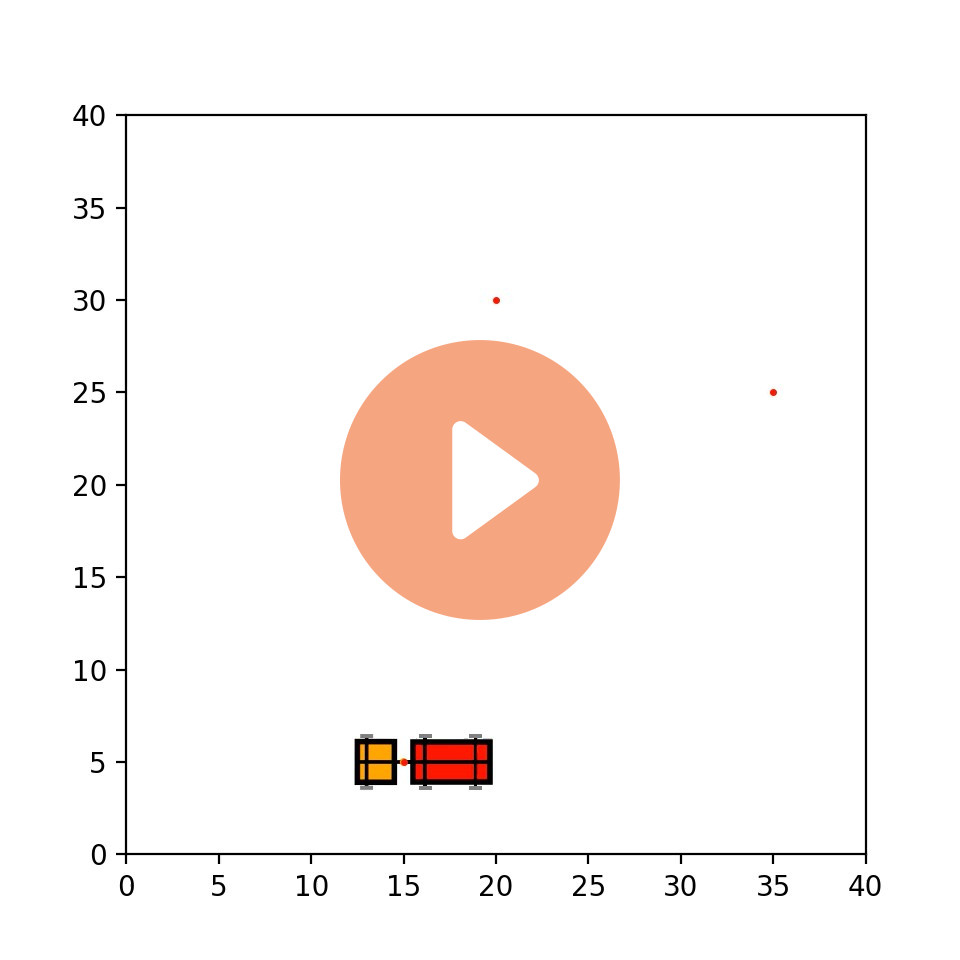
\includegraphics[width=0.8\textwidth]{images/thumb3}}%
        {videos/movie3.mp4}
\end{minipage}

\footnotesize{Available at \url{https://github.com/martimunicoy/TrailerController}}

\end{onlyenv}

\end{frame}


%-----------------------------------------------------------------
% \subsection{Optimisation-based}

% \begin{frame}{Optimisation-based}
% \begin{figure}[H]
%     \centering
%     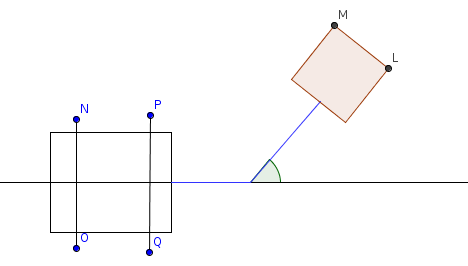
\includegraphics[width=0.55\textwidth]{images/pic_trailer.png}
%     \caption{Geometric situation}
%     \label{fig:trailer}
% \end{figure}

% \begin{figure}[H]
%     \centering
%     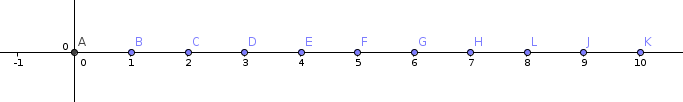
\includegraphics[width=0.55\textwidth]{images/divisions.png}
%     \caption{Time divisions of the method}
%     \label{fig:trailer2}
% \end{figure}
% \end{frame}

% \begin{frame}{Frame Title}
% We optimise, as a function of $\delta$:
% $$
% cost_{\alpha}(y, \phi) = y^2+\alpha \phi^2 
% $$

% \end{frame}


%-----------------------------------------------------------------

% \subsection{Experience Control}
% \begin{frame}{First Tests of the Model}

% \begin{onlyenv}<1>
% \begin{minipage}{.5\textwidth}
%     \begin{figure}[H]
%         \centering
%         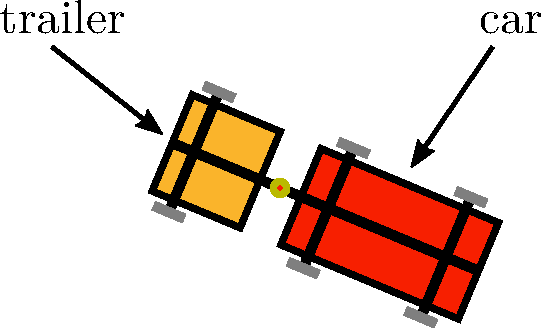
\includegraphics[width=0.6\textwidth]{images/car-trailer}
%         \caption{Diagram of the system}
%         \label{fig:car-trailer-diag}
%     \end{figure}
%     \begin{itemize}
%         \item Go from $A$ to $B$ backwards.
%     \end{itemize}
% \end{minipage}%
% \begin{minipage}{0.5\textwidth}
%     \begin{figure}[H]
%         \centering
%         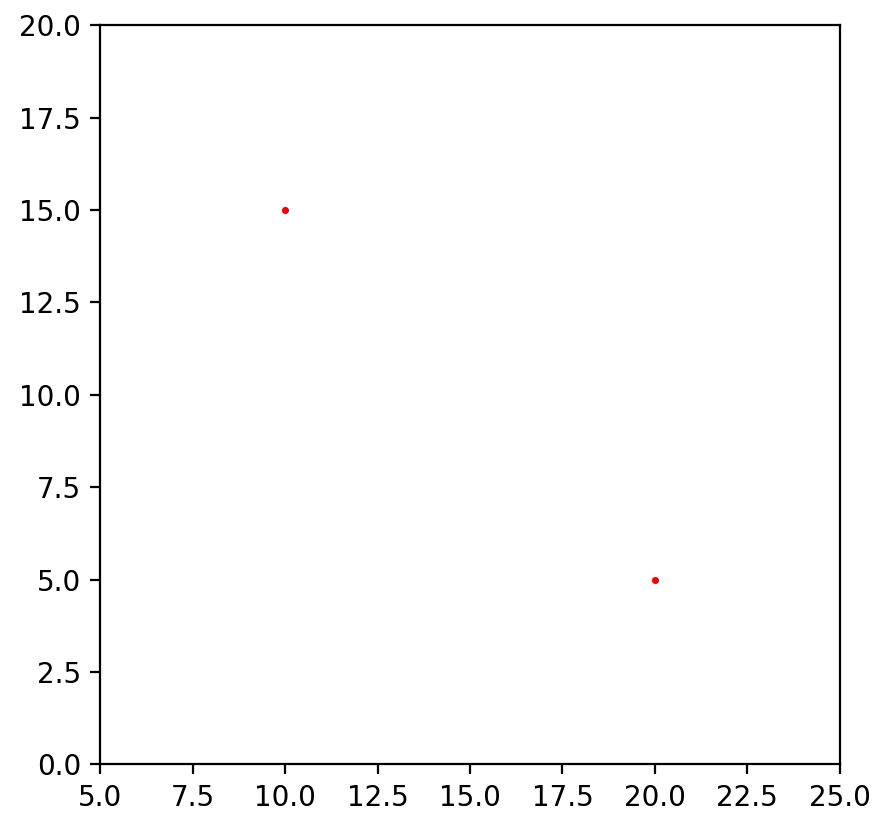
\includegraphics[width=\textwidth]{images/points}
%         % \caption{Diagram of the system}
%         \label{fig:points}
%     \end{figure}
% \end{minipage}
% \end{onlyenv}

% \begin{onlyenv}<2>
% \begin{minipage}{.5\textwidth}
%     \movie[width=6cm,height=4.5cm,poster]{%
%         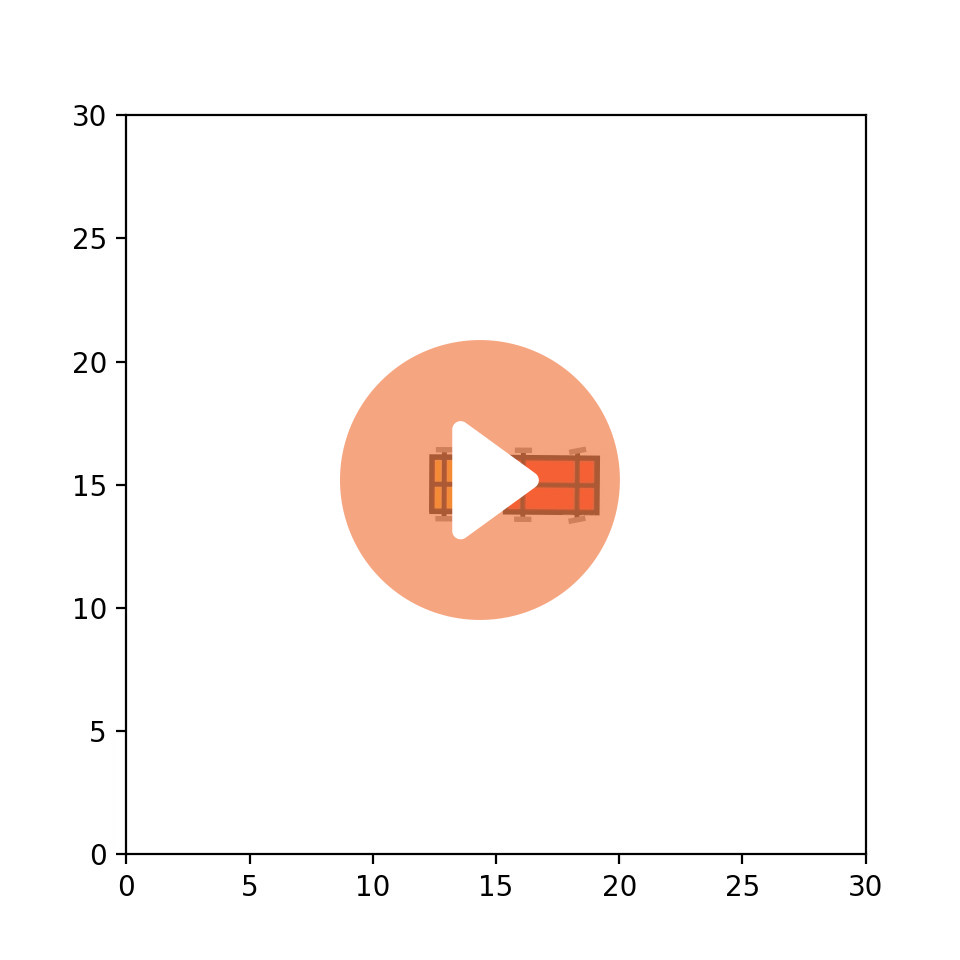
\includegraphics[width=0.8\textwidth]{images/thumbtest1}}%
%         {videos/test.mp4}
% \end{minipage}%
% \begin{minipage}{.5\textwidth}
%     \movie[width=6cm,height=4.5cm,poster]{%
%         \hspace{0.8cm}%
%         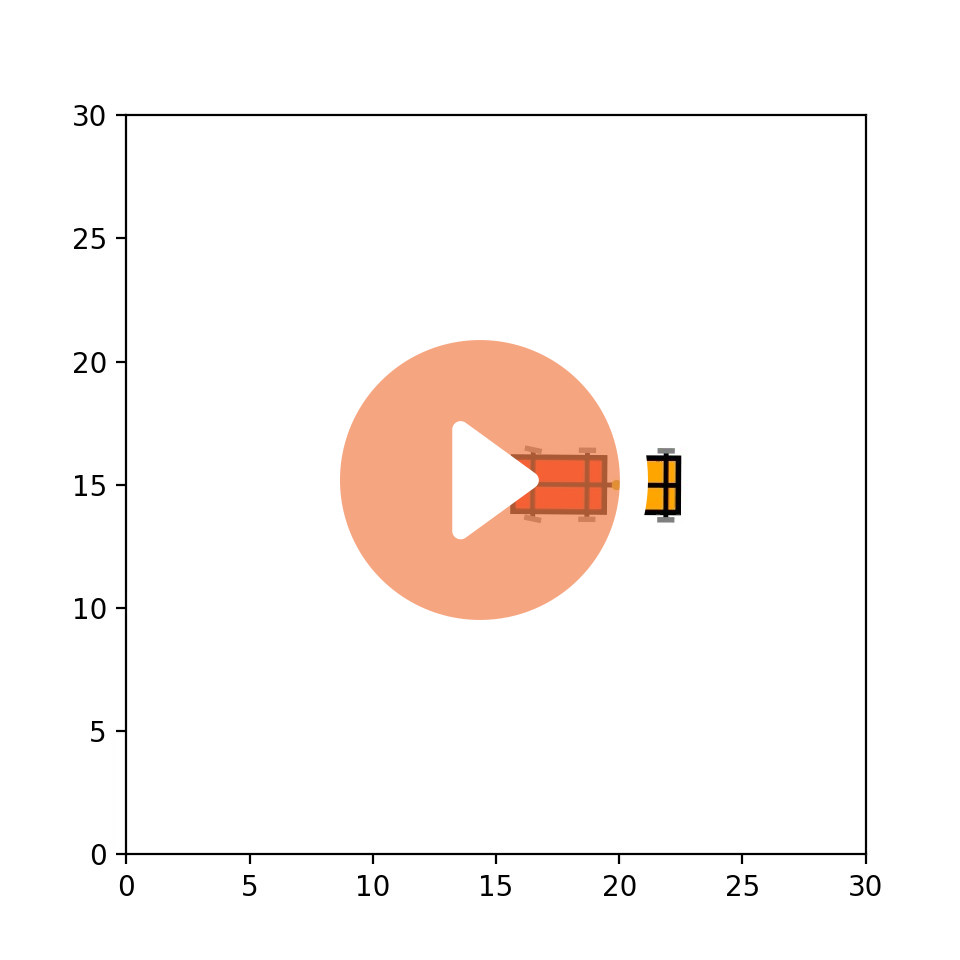
\includegraphics[width=0.8\textwidth]{images/thumbtest2}}%
%         {videos/test2.mp4}
% \end{minipage}
% \end{onlyenv}

% \end{frame}

% \begin{frame}{Steering-based Control}

% \begin{onlyenv}<1-4>
% \begin{minipage}{.45\textwidth}
%     \begin{enumerate}[(i)]
%         \footnotesize
%         \item<2,4> Face trailer to a “non-annoying” direction.
%         \item<3,4> Move the car to the goal point.
%     \end{enumerate}
%     \begin{itemize}
%         \item<4> Keep repeating (i) until reaching point $B$.
%     \end{itemize}
% \end{minipage}%
% \begin{minipage}{.55\textwidth}
%     \begin{onlyenv}<1>
%     \begin{figure}[H]
%         \centering
%         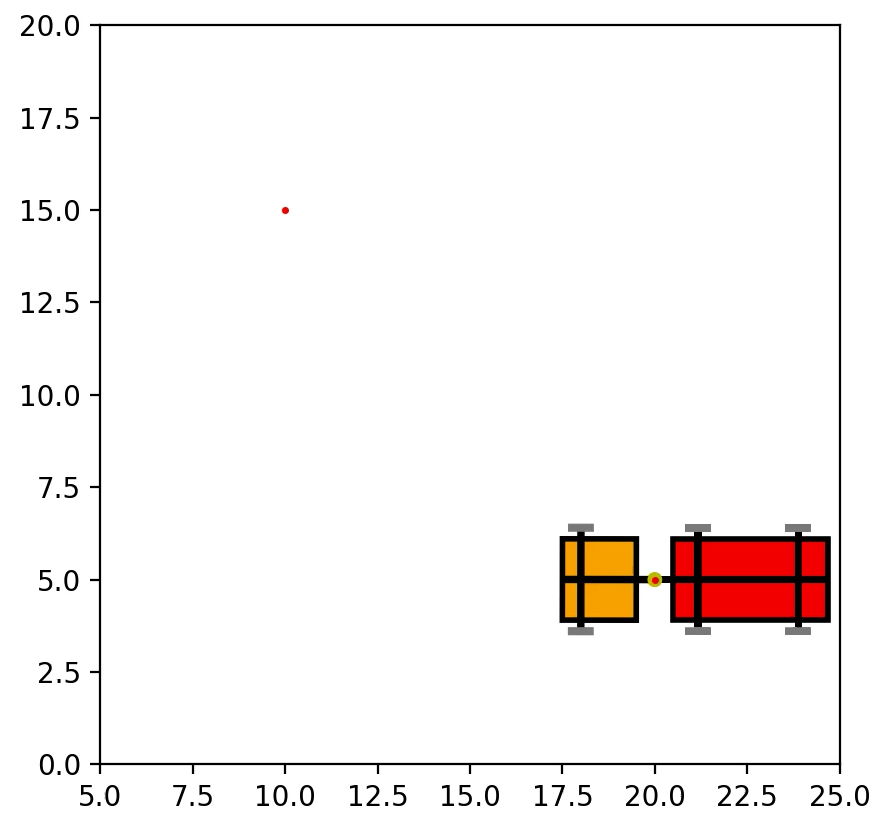
\includegraphics[width=\textwidth]{images/snapshot1}
%         % \caption{Diagram of the system}
%         \label{fig:points}
%     \end{figure}
%     \end{onlyenv}
%     \begin{onlyenv}<2>
%     \begin{figure}[H]
%         \centering
%         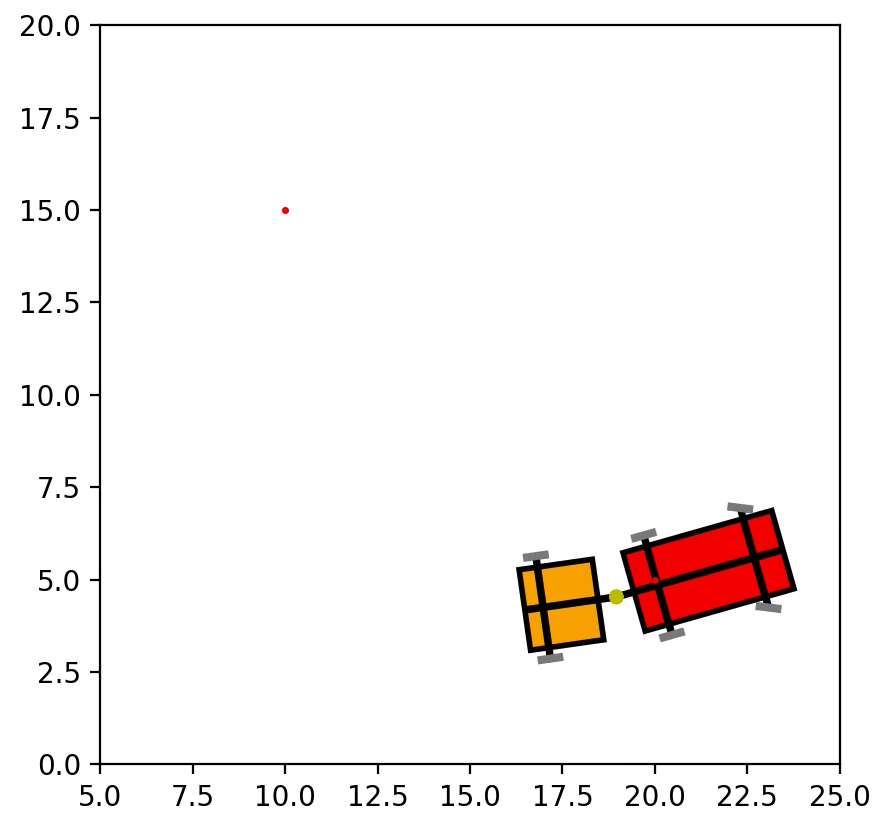
\includegraphics[width=\textwidth]{images/snapshot2}
%         % \caption{Diagram of the system}
%         \label{fig:points}
%     \end{figure}
%     \end{onlyenv}
%     \begin{onlyenv}<3>
%     \begin{figure}[H]
%         \centering
%         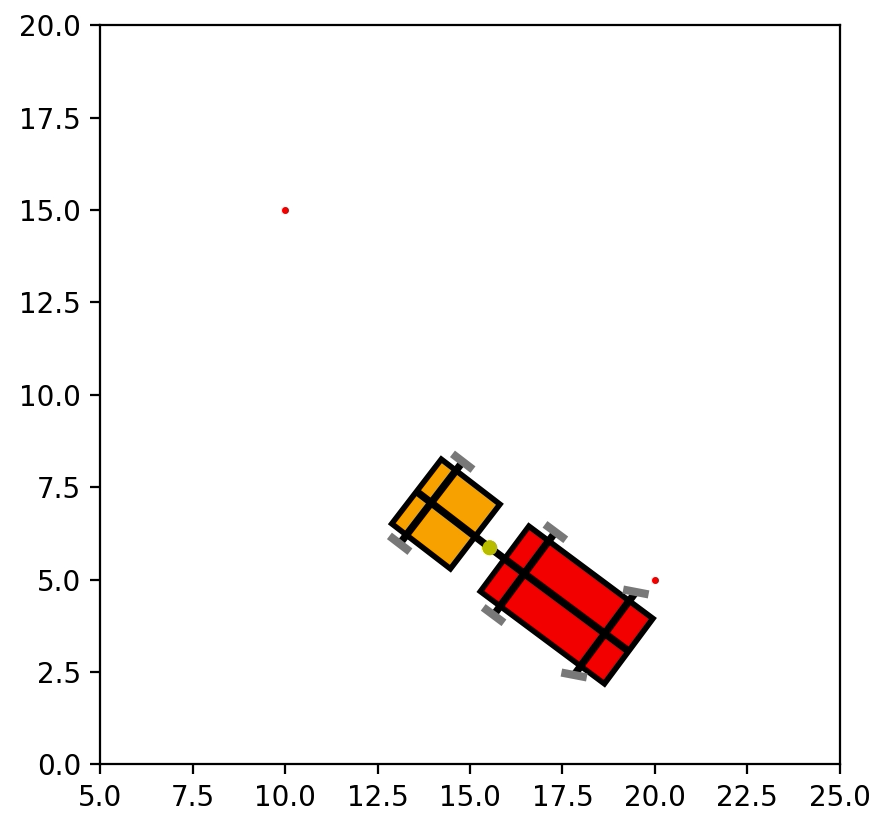
\includegraphics[width=\textwidth]{images/snapshot3}
%         % \caption{Diagram of the system}
%         \label{fig:points}
%     \end{figure}
%     \end{onlyenv}
%     \begin{onlyenv}<4>
%     \movie[width=7cm,height=5.25cm,poster]{%
%         \hspace{0.8cm}%
%         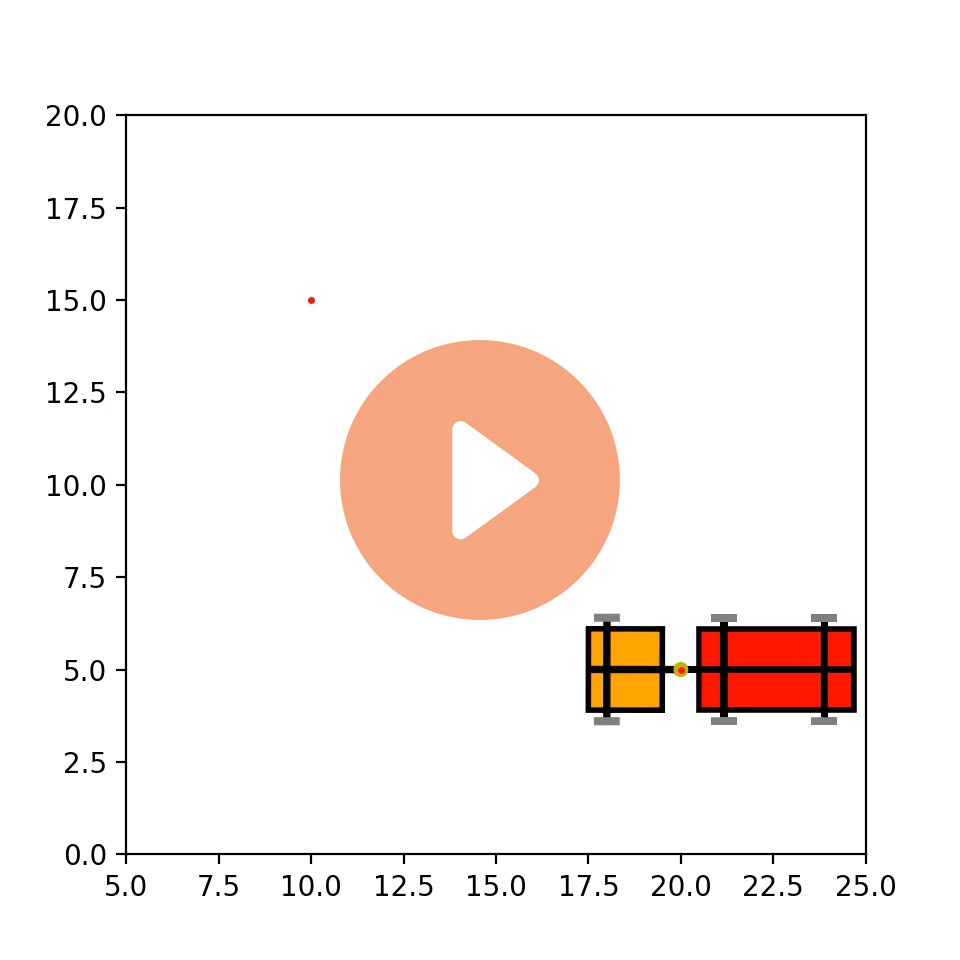
\includegraphics[width=0.8\textwidth]{images/thumb1}}%
%         {videos/movie1.mp4}
%     % \begin{figure}[H]
%     %     \centering
%     %     \movie[width=7cm,height=5.25cm,poster]{%
%     %     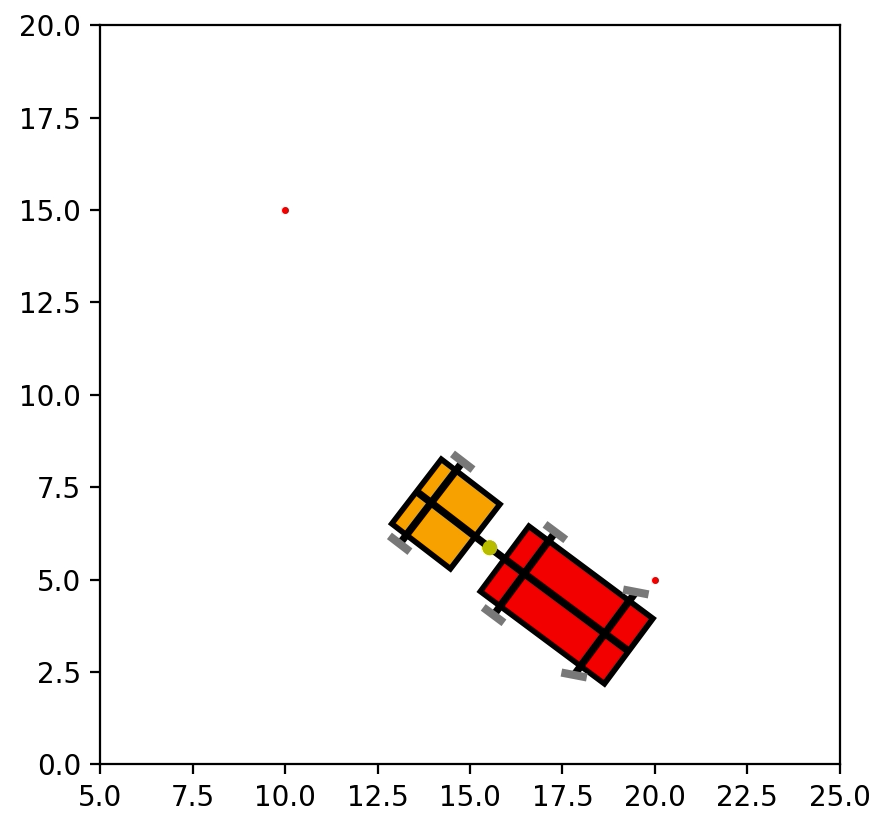
\includegraphics[width=\textwidth]{images/snapshot3}}%
%     %     {videos/movie1.mp4}
%     %     \label{fig:points}
%     % \end{figure}
%     \end{onlyenv}
% \end{minipage}
% \end{onlyenv}

% \begin{onlyenv}<5>
% \begin{minipage}{.5\textwidth}
%     \movie[width=6cm,height=4.5cm,poster]{%
%         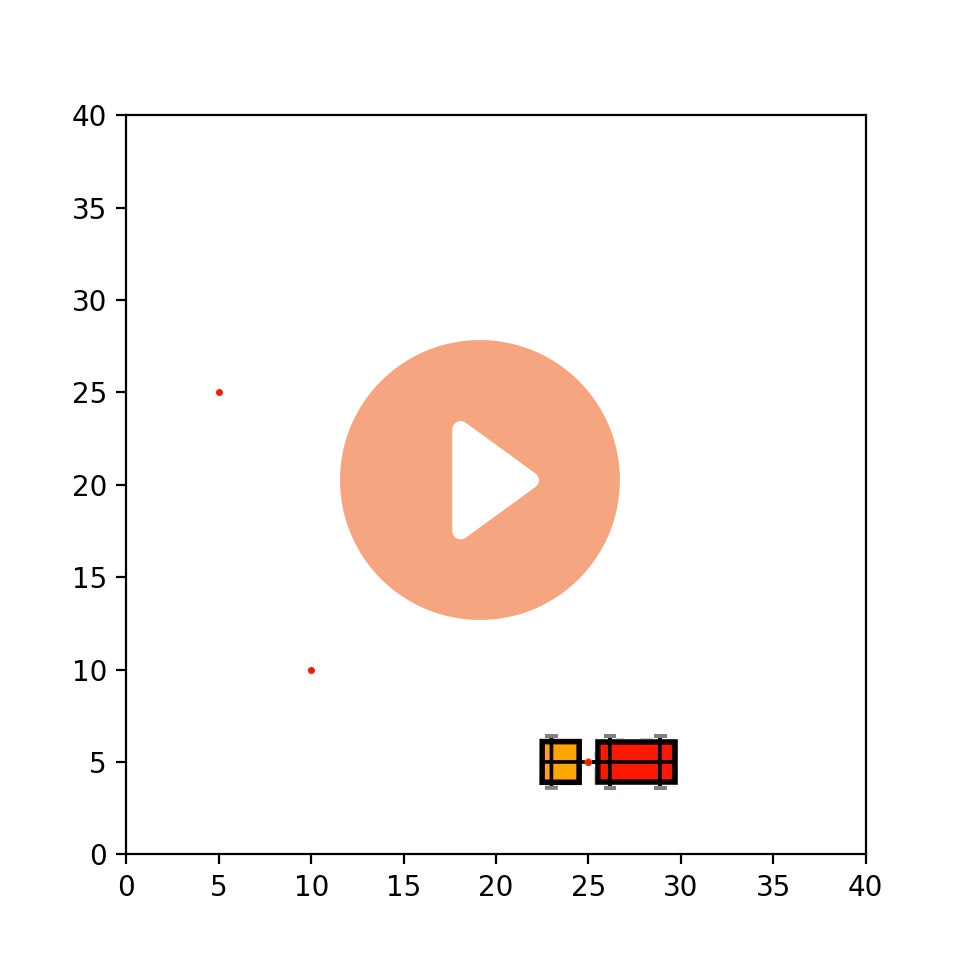
\includegraphics[width=0.8\textwidth]{images/thumb2}}%
%         {videos/movie2.mp4}
% \end{minipage}%
% \begin{minipage}{.5\textwidth}
%     \movie[width=6cm,height=4.5cm,poster]{%
%         \hspace{0.8cm}%
%         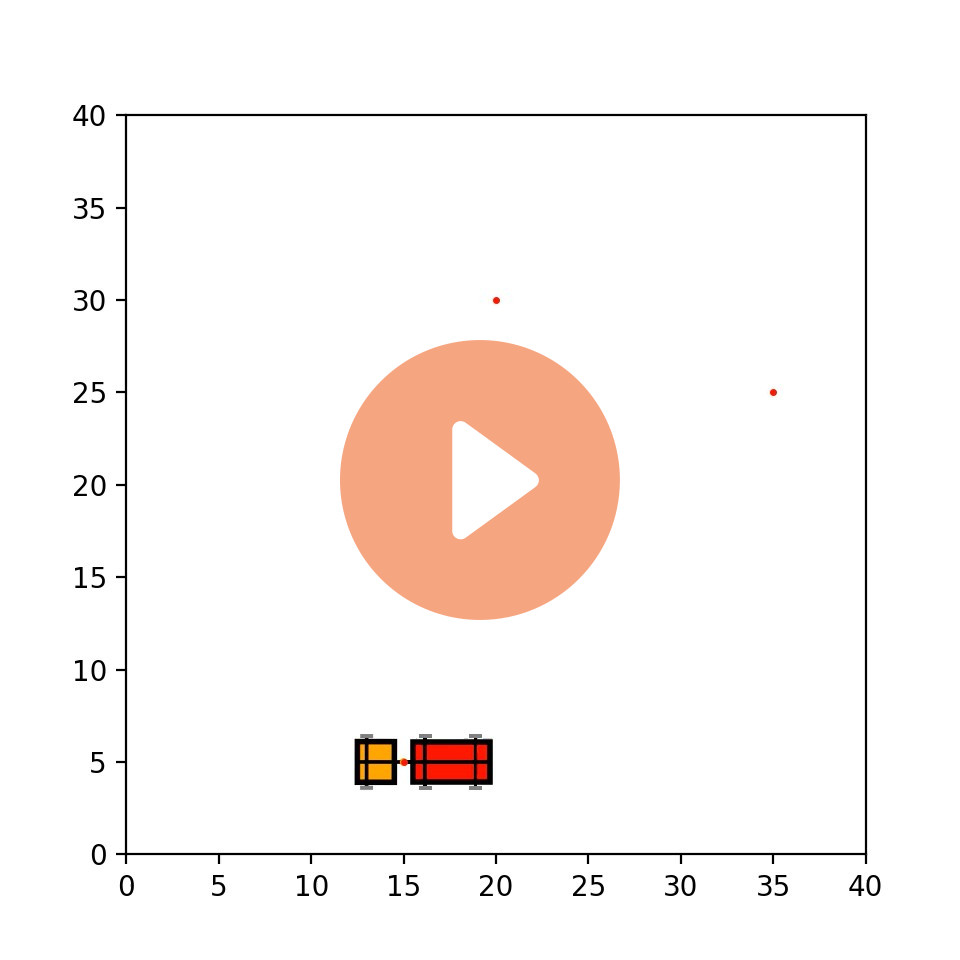
\includegraphics[width=0.8\textwidth]{images/thumb3}}%
%         {videos/movie3.mp4}
% \end{minipage}
% \end{onlyenv}

% \end{frame}
% \input{contents/4-experience}
%-----------------------------------------------------------------
%	CONCLUSIONS
%	!TEX root = ./main.tex
%-----------------------------------------------------------------
\section{Conclusions}
\begin{frame}{Conclusions}
We saw three different approaches:
\begin{itemize}
    \item Controller using pole placement (using MATLAB).
    \item Optimisation-based control (using C).
    \item Steering-based control (using Python).
\end{itemize}
All of them are viable options for control with their own advantages and disadvantages.
\end{frame}

%-----------------------------------------------------------------
\appendix
\begin{frame}{References}
% \begin{frame}[allowframebreaks]{References}
	\def\newblock{}
	\nocite{Nilsson2013}
	\nocite{steering}
	\nocite{jack}
	\nocite{Sontag1998}
	\nocite{Hinrichsen2005}
	\nocite{Hautus2001}
	\printbibliography[heading=bibintoc]
\end{frame}

\end{document}

